\documentclass[11pt]{scrartcl}
\usepackage[sexy]{evan}

\usepackage{answers}
\Newassociation{hint}{hintitem}{all-hints}
\renewcommand{\solutionextension}{out}
\renewenvironment{hintitem}[1]{\item[\bfseries #1.]}{}

\begin{document}
\title{Lógica}
\author{Ricardo Largaespada}
\date{27 Enero 2024}

\maketitle

\section{Introducción}

En los últimos años, la participación en competiciones internacionales de matemáticas ha mejorado significativamente. Una de las consecuencias del éxito de nuestros estudiantes es el crecimiento en la demanda de personas interesadas en aprender más sobre lo que es la olimpiada y qué tipo de problemas se abordan en sus competiciones.

La característica distintiva de los problemas de la olimpiada de matemáticas en comparación con los problemas habituales es su alto nivel de exigencia en el uso del razonamiento lógico. Por lo tanto, en muchos casos, la matemática se presenta como una herramienta para desarrollar la argumentación de ideas abstractas.

Este es la primera de dos clases con el objetivo de presentar dichos problemas, incluso sin desarrollar una teoría matemática propiamente dicha. Nos enfocaremos directamente en las ideas.

\section{Problemas Resueltos}
\begin{example}
Cuatro chicos juegan al tiro al blanco. Cada uno de ellos disparó tres veces. En el blanco a continuación, se pueden ver los lugares alcanzados. La puntuación es 6 para el centro y disminuye un punto por cada nivel más distante.
\begin{center}
    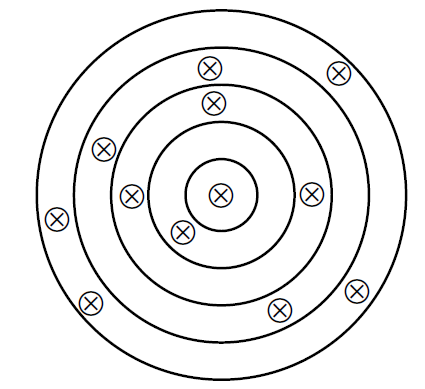
\includegraphics[scale=0.5]{clase_01_diana.png}
\end{center}
Si los cuatro chicos empataron, determina:\begin{itemize}
\item[(a)] La puntuación total de cada jugador.
\item[(b)] La puntuación de los tres tiros de cada jugador.
\end{itemize}
\end{example}
La suma de todos los puntos obtenidos fue $6+5+4\times 3+3\times 3+2\times 4 = 40$. Como todos empataron, cada persona debe haber obtenido exactamente 10 puntos (esto responde al punto a). También es importante darse cuenta de que nadie falló ninguno de sus tiros, ya que hay exactamente 12 dardos en la diana. 

Observa que uno de los jugadores (digamos A) ha acertado uno de los dardos en el centro de la diana, consiguiendo 6 puntos. Para completar los 10 puntos debe haber anotado 4 puntos más. Como es imposible que haya conseguido sólo 1 punto, o que haya fallado, nos queda la posibilidad de que haya conseguido 2 puntos en los otros dos tiros. (Continuar con la solución)

El objetivo de otro tipo de problemas es encontrar un ejemplo que cumpla alguna propiedad.

\begin{example}
Encuentra una forma de escribir los dígitos del 1 al 9 en secuencia de manera que los números determinados por dos dígitos consecutivos cualesquiera sean divisibles por 7 ó 13.
\end{example}

En primer lugar, vamos a enumerar todos los números de dos cifras que son múltiplos de 7 o de 13. Son los siguientes.\\
Múltiplos de 7: 14, 21, 28, 35, 42, 49, 56, 63, 70, 77, 84, 91, 98.\\
Múltiplos de 13: 13, 26, 39, 52, 65, 78, 91\\

Como no podemos repetir ningún dígito, tenemos que descartar 77. Por otra parte, ninguno de los números de la lista (excluyendo el 77) termina en 7. A partir de aquí, podemos estar seguros de que el primer número de la lista debe ser el 7. Para averiguar las posibles listas, utilizamos un diagrama de ``árbol'':

\begin{center}
    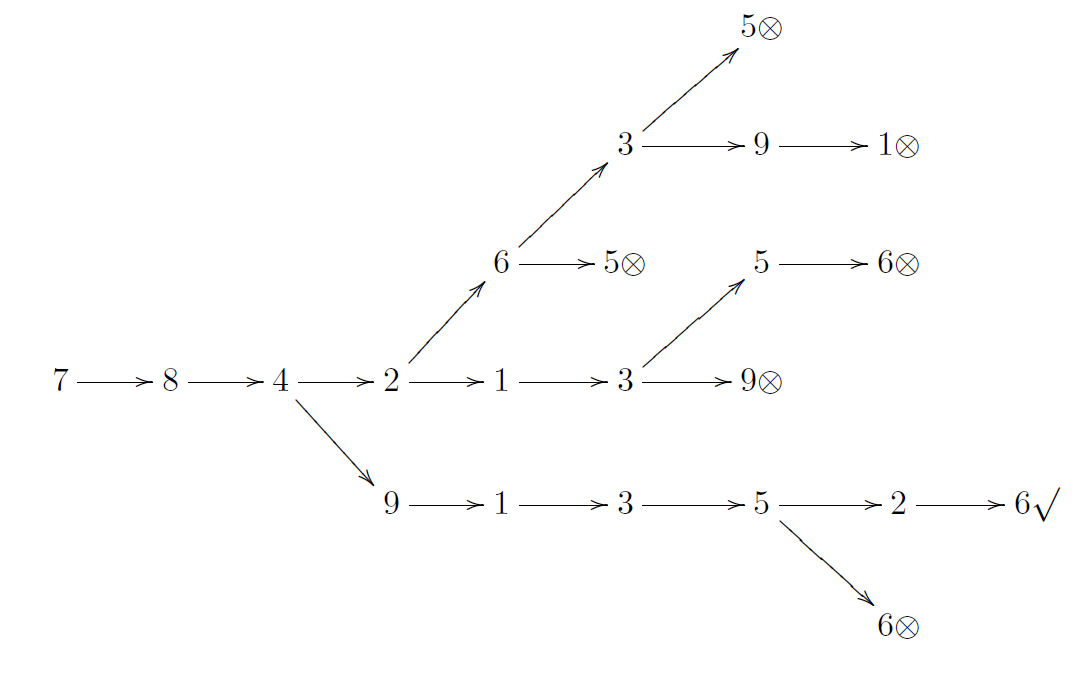
\includegraphics[scale=0.5]{clase_01_diagrama_arbol.png}
\end{center}
Representamos con una \(\bigotimes\) cuando no era posible continuar la lista sin repetir ningún dígito. Así, la forma correcta de escribir los dígitos es: 784913526.

En algunos casos es necesario utilizar variables para resolver un problema. Esto se debe a que hay información no especificada en el enunciado, y el uso de letras es una forma inteligente y fácil de trabajar con valores desconocidos.

\begin{example}[Rusia 1995]
Un tren sale de Moscú a las $x$ horas e $y$ minutos y llega a Saratov a las $y$ horas y $z$ minutos. La duración del viaje fue de $z$ horas y $x$ minutos. Encuentre todos valores posibles de $x$.    
\end{example}
A partir de las condiciones del problema, tenemos que:
\[(60y+z)-(60x+y)=60z+x\Rightarrow 60(y-z-x)=x+y-z.\]
Esto garantiza que $x + y - z$ es múltiplo de 60. Por otra parte, como $0\le x, y, z\le 23$, el único valor posible para $x + y - z$ es 0. En otras palabras, $x + y = z$. Además, en la ecuación inicial tenemos que $60(y - x - z) = 0$. Por tanto, $y = x + z$. Por tanto, el único valor de $x$ que garantiza estas igualdades es $x = 0$.\\

Es importante darse cuenta de que en el ejemplo anterior el uso de letras por sí solo no era suficiente para resolver el problema. La clave para resolver las ecuaciones anteriores era el significado de las letras: números enteros entre 0 y 60. Sin esta restricción, el problema presentaría infinitas soluciones. Así que éste es el consejo: nunca olvides el significado de las variables que estás utilizando, ya sean dígitos, números enteros, números racionales o cualquiera que sea la propiedad. Recuerda que esta propiedad jugará un papel importante en la resolución del problema.

Organizar la información también es útil en la mayoría de los problemas, como veremos en el siguiente ejemplo.
ejemplo siguiente.

\begin{example}
    Paul tiene 13 cajas rojas y cada una de ellas está vacía o contiene 7 cajas azules. Cada caja azul está vacía o contiene 7 cajas verdes. Si tiene 145 cajas vacías, ¿cuántas cajas tiene en total?
\end{example}
Elaboremos una tabla que nos ayude a resolver el problema:

\begin{center}
\begin{tabular}{|c|c|c|c|}
\hline
 & Rojo & Azul & Verde \\
\hline
Lleno & $x$ & $y$ & $0$ \\
\hline
Vacío & $13 - x$ & $7x - y$ & $7y$ \\
\hline
Total & $13$ & $7x$ & $7y$ \\
\hline
\end{tabular}
\end{center}

Supongamos que el número de cajas rojas llenas es $x$ y el número de cajas azules llenas es $y$. Entonces tenemos $7x$ cajas azules y $7y$ cajas verdes. Observa también que todas las cajas verdes están vacías. Por lo tanto, el número total de cajas vacías es $(13-x) + (7x-y) + 7y = 145$. Por lo tanto, podemos concluir que $x+y = 22$. Como el número total de cajas es $13 + 7(x+y)$, la respuesta correcta es $13 + 7 \times 22 = 167$.

\Opensolutionfile{all-hints}

\section{Problemas Propuestos}
\begin{problem}
    Carlos tiene tres hermanos más que hermanas. Carla, la hermana de Carlos, tiene el doble de hermanos que de hermanas. ¿Cuántos hijos (hombres y mujeres) tiene el padre de Carlos y Carla?
    \begin{hint}
        Llamemos $V$ y $M$ al número de hijos e hijas del papá de Carlos. Intenta escribir las relaciones correspondientes.
    \end{hint}
\end{problem}

\begin{problem}
    En un hotel para perros y gatos, el 10\% de los perros se creen gatos y el 10\% de los gatos se creen perros. gatos piensan que son perros. También descubrimos que el 20\% de los animales piensan que son gatos. Si hay 10 gatos en el hotel, ¿cuántos son perros?
    \begin{hint}
        Construye una tabla, ¡intenta utilizar una sola variable!
    \end{hint}
\end{problem}

\begin{problem}
    ¿Es posible cortar un tablero de $39 \times 55$ en varios rectángulos de $5 \times 11$?
    \begin{hint}
        No. Demuestre que no es posible cubrir un lado del tablero.
    \end{hint}
\end{problem}

\begin{problem}
    A finales de 2011, Ricardo tenía un cuarto de edad que su abuelo. La suma de sus años de nacimiento es 3927. ¿Cuántos años tenía Ricardo en 2024?
    \begin{hint}
        Sea \( J \) la edad de Ricardo en 2011 y \( A \) la edad de su abuelo en 2011.
        Utiliza las condiciones dadas: \( J = \frac{1}{4}A \) y \( (2011 - J) + (2011 - A) = 3927 \).
    \end{hint}
\end{problem}

\begin{problem}
    Un profesor propone 80 problemas a un alumno, informándole de que gana 5 puntos si acierta cada problema y pierde 3 puntos si no lo resuelve. Al final, el alumno obtuvo 8 puntos. ¿Cuántos problemas resolvió correctamente?
    \begin{hint}
        Sea \(x\) el número de problemas resueltos correctamente. Utiliza la ecuación: \(5x - 3(80 - x) = 8\). Simplifica y resuelve para encontrar el valor de \(x\).
    \end{hint}
\end{problem}

\begin{problem}
    En una isla hay cuatro tipos de billetes: 1\$,
10\$, 100\$ y 1000\$. ¿Podemos conseguir 1 millón de dólares con exactamente 500.000 billetes?
    \begin{hint}
        Sean \(x\), \(y\), \(z\), y \(w\) el número de notas. Establece un sistema con dos ecuaciones y utiliza el hecho de que \(500,000\) no es múltiplo de \(9\).
    \end{hint}
\end{problem}

\begin{problem}
    Tienes una lista de números reales cuya suma es 40. Si cambias cada número $x$ de la lista por $1-x$, la suma de los nuevos números será 20. Ahora, si sustituyes cada número $x$ por $1 + x$, ¿cuál será la suma?
    \begin{hint}
        Denota los números originales como \(x_1, x_2, \ldots, x_n\), con una suma total de 40.
    \end{hint}
\end{problem}

\begin{problem}
Completa la siguiente tabla para que:
\begin{enumerate}
    \item La suma de tres vecinos cualesquiera sea igual.
    \item La suma total de los números sea 171.
\end{enumerate}

\begin{center}
\begin{tabular}{|*{14}{>{\centering\arraybackslash}p{1em}|}}
\hline
 & & & & 15 & & & & 13 & & & & & \\
\hline
\end{tabular}
\end{center}
\begin{hint}
    Considera los bloques de tres vecinos.
\end{hint}
\end{problem}

\begin{problem}
    Trabajando juntos, A y B pintan una casa en tres días; B y C pintan la misma casa en cuatro días; A y C en seis días. Si los tres trabajan trabajan juntos, ¿cuántos pintarán la casa en cuántos días?
    \begin{hint}
        Usa el hecho de que A y B pintaron un tercio de la casa en un día.
    \end{hint}
\end{problem}

\begin{problem}
    Se coloca un número secreto en cada casilla de un tablero de $4 \times 4$. Se sabe que la suma de los números de cada fila, columna y diagonal es 1. Con esta información, ¿es posible determinar la suma de los números escritos en las cuatro esquinas? ¿Y la suma de los cuatro números escritos en el centro? En caso afirmativo, ¿cuáles son estas sumas?
    \begin{hint}
        Separa el tablero en tres regiones. No te preocupes por los números, sino por la suma de los números en estas regiones inteligentes.
    \end{hint}
\end{problem}

\Closesolutionfile{all-hints}

\section{Sugerencias}
\begin{enumerate}
\input{all-hints.out}
\end{enumerate}

\end{document}